%%%%%%%%%%%%%%%%%%%%%%%%%%%%%%%%%%%%%%%%%%%%%%%%%%%%%%%%%%%%
%%  This Beamer template was created by Cameron Bracken.
%%  Anyone can freely use or modify it for any purpose
%%  without attribution.
%%
%%  Last Modified: January 9, 2009
%%

\documentclass[xcolor=x11names,compress]{beamer}

%% General document %%%%%%%%%%%%%%%%%%%%%%%%%%%%%%%%%%
\usepackage{hyperref}
\usepackage{graphicx}
\usepackage{tikz}
\usetikzlibrary{decorations.fractals}
\usetikzlibrary{shadings}
%%%%%%%%%%%%%%%%%%%%%%%%%%%%%%%%%%%%%%%%%%%%%%%%%%%%%%


%% Beamer Layout %%%%%%%%%%%%%%%%%%%%%%%%%%%%%%%%%%
%\useinnertheme{rounded}
%\usefonttheme{serif}
%\usepackage{palatino}
%\usetheme{Madrid}
\useoutertheme[subsection=false,shadow, circles]{smoothbars}
\usecolortheme{rose}

\usepackage{fontspec}
\usepackage{xunicode} 
\usepackage{xltxtra}
\usepackage[ruled, vlined]{algorithm2e}

\usefonttheme{serif}
% (commenting this out to run on writelatex.com) 
\setmainfont{FlamaLight}


\setbeamerfont{title like}{shape=\scshape}
\setbeamerfont{frametitle}{shape=\scshape}

\setbeamercolor*{lower separation line head}{bg=DeepSkyBlue4} 
\setbeamercolor*{normal text}{fg=black,bg=white} 
\setbeamercolor*{alerted text}{fg=red} 
\setbeamercolor*{example text}{fg=black} 
\setbeamercolor*{structure}{fg=black} 
 
\setbeamercolor*{palette tertiary}{fg=black,bg=black!10} 
\setbeamercolor*{palette quaternary}{fg=black,bg=black!10} 

\renewcommand{\(}{\begin{columns}}
\renewcommand{\)}{\end{columns}}
\newcommand{\<}[1]{\begin{column}{#1}}
\renewcommand{\>}{\end{column}}
%%%%%%%%%%%%%%%%%%%%%%%%%%%%%%%%%%%%%%%%%%%%%%%%%%

\newtheorem{thm}{Theorem}
\newtheorem{pf}{Proof}
\newtheorem{defn}{Definition}
\newtheorem{rmk}{Remark}


\begin{document}


%%%%%%%%%%%%%%%%%%%%%%%%%%%%%%%%%%%%%%%%%%%%%%%%%%%%%%
%%%%%%%%%%%%%%%%%%%%%%%%%%%%%%%%%%%%%%%%%%%%%%%%%%%%%%
%\section{\scshape Introduction}
\begin{frame}
\title{Julia Sets}
\subtitle{Theory and Algorithms}
\author{
	Josh Lipschultz \& Ricky LeVan\\
	{\it MATH/CAAM 435}\\
}
\date{
%	\begin{tikzpicture}[decoration=Julia set] 
%		\draw[DeepSkyBlue4] decorate{ decorate{ decorate{ (0,0) -- (3,0) }}}; 
%	\end{tikzpicture} 
\begin{tikzpicture}[decoration=Cantor set,very thick]
\draw[DeepSkyBlue4] decorate{ (0,0) -- (5,0) };
\draw[DeepSkyBlue4] decorate{ decorate{ (0,-.5) -- (5,-.5) }};
\draw[DeepSkyBlue4] decorate{ decorate{ decorate{ (0,-1) -- (5,-1) }}};
\draw[DeepSkyBlue4] decorate{ decorate{ decorate{ decorate{ (0,-1.5) -- (5,-1.5) }}}};
\end{tikzpicture}
	\\
	\vspace{1cm}
	April 15, 2014
}
\titlepage
\end{frame}

%%%%%%%%%%%%%%%%%%%%%%%%%%%%%%%%%%%%%%%%%%%%%%%%%%%%%%
%%%%%%%%%%%%%%%%%%%%%%%%%%%%%%%%%%%%%%%%%%%%%%%%%%%%%%
%\begin{frame}{Introduction}
%\tableofcontents
%\end{frame}

%%%%%%%%%%%%%%%%%%%%%%%%%%%%%%%%%%%%%%%%%%%%%%%%%%%%%%
%%%%%%%%%%%%%%%%%%%%%%%%%%%%%%%%%%%%%%%%%%%%%%%%%%%%%%
\section{\scshape Preliminaries}
\subsection{frame 1}
\begin{frame}

Quick refresher from last time:

\pause

\begin{defn}
The \textsl{stable set} of a a complex polynomial $P: \mathbb{C} \rightarrow \mathbb{C}$, denoted $S(P)$, is the complement of $J(C)$.
\end{defn}

\pause

\begin{defn}
An orbit is \textsl{bounded} if there exists a $K$ such that $|Q_c^{\circ n}(z)| < K$ for all $n$. Otherwise the orbit is \textsl{unbounded}.
\end{defn}

\pause

\begin{rmk}
The points of $S^1$ are \textsl{supersensitive} under $Q_{0}$. That is, any open ball $B$ around $z \in S^1$ has the property that $\bigcup_{n=0}^\infty Q_0^{\circ n} (B) = \mathbb{C} \setminus \{p\}$ for at most one point $p$.
\end{rmk}

\end{frame}

%%%%%%%%%%%%%%%%%%%%%%%%%%%%%%%%%%%%%%%%%%%%%%%%%%%%%%
%%%%%%%%%%%%%%%%%%%%%%%%%%%%%%%%%%%%%%%%%%%%%%%%%%%%%%

\subsection{frame 2}
\begin{frame}

\begin{defn}
The Julia Set $J_c$ is the boundary of the filled Julia set $K_c$. (The filled Julia set is the set of bounded points of $Q_c$.) We could alternatively define $J_c$ as the closure of the set of repelling points of $Q_c$.
\end{defn}

\pause


\begin{rmk}
For the quadratic map $Q_0(z) = z^2$ we saw chaotic behavior only on $S^1$ by angle doubling ($\theta \rightarrow 2\theta$). We also saw that $|Q_0(z)| \rightarrow \infty$ for all $|z| > 1$ and $|Q_0(z)| \rightarrow 0$ for all $|z| < 1$.
\end{rmk}

\pause


\begin{rmk}
Finally, we learned that for $Q_{-2}(z) = z^2 - 2$, we have $J_2 = K_2 = [-2, 2]$, so any $z \in \mathbb{C} \setminus [-2,2] \rightarrow \infty$ as we compose $Q_{-2}(z)$ infinitely many times. 
\end{rmk}

\end{frame}

%%%%%%%%%%%%%%%%%%%%%%%%%%%%%%%%%%%%%%%%%%%%%%%%%%%%%%
%%%%%%%%%%%%%%%%%%%%%%%%%%%%%%%%%%%%%%%%%%%%%%%%%%%%%%

\subsection{frame 3}
\begin{frame}

\begin{defn}
A set $\Lambda \subseteq \mathbb{C}$ is a Cantor set if it is a closed, totally disconnected, and perfect subset of $\mathbb{C}$. (Adapted from the version for an interval of the real line.)
\end{defn}

\end{frame}




%%%%%%%%%%%%%%%%%%%%%%%%%%%%%%%%%%%%%%%%%%%%%%%%%%%%%%
%%%%%%%%%%%%%%%%%%%%%%%%%%%%%%%%%%%%%%%%%%%%%%%%%%%%%%
\section{\scshape Cantor Construction}


\subsection{frame 2}
\begin{frame}

\begin{itemize}
\item Goal: discuss and prove parts of:
\end{itemize}

\vspace{1cm}

\begin{theorem}
If $|c|$ is sufficiently large, $\Lambda$, the set of points whose entire forward orbits lie within the circle $|z|=|c|$, is a Cantor set on which $Q_c$ is topologically conjugate to the shift map on two symbols. All points in $\mathbb{C} - \Lambda$ tend to $\infty$ under iteration of $Q_c$. Hence, $J_c=K_c$.
\end{theorem}

\end{frame}


\subsection{frame 2}
\begin{frame}

\begin{theorem} [The Escape Criterion]
Suppose $2 < |c| \le |z|$. Then we have that $|Q_c^{\circ n}(z)| \rightarrow \infty$ as $n \rightarrow \infty$.
\end{theorem}

\begin{proof}
We use the triangle inequality to get the following estimate:
\begin{equation}
    |Q_c(z)| \geq |z|^2 - |c| \geq |z|^2 - |z| = |z|(|z|-1)
\end{equation}
Since $|z| > 2$, we know that $|z|-1>1$, so there exists $\lambda > 0$ such that 
\begin{equation}
    |Q_c^n(z)| \geq (1+\lambda)^n|z|
\end{equation}
Since $|z|$ is fixed and $(1+\lambda)^n$ grows arbitrarily large, $|Q_c^n(z)|$ also grows arbitrarily large, as desired.
\end{proof}

\end{frame}

\subsection{frame 3}
\begin{frame}

\begin{theorem}
Let $D$ be the closed disk (i.e. $\{z : |z| \le |c|\}$), with $|c|>2$. Then the filled Julia set of $Q_c$ is given by
\begin{align*}
K_c = \bigcap\limits_{n\ge 0} Q_c^{\circ -n} (D)
\end{align*}
where $Q_c^{\circ -n} (D)$ denotes the preimage of $D$ under $Q_c^{\circ n}$
\end{theorem}

\begin{proof}
    Consider the case where
    $z\notin \bigcap_{n\ge 0} Q_c^{\circ -n} (D)$.
    Then there exists some $k\in \mathbb{N}$ such that $z\notin Q_c^{\circ -k} (D)$,
    so we have that $Q_c^{\circ k}(z) \notin D$. 
    Thus by the escape criterion, $z$ escapes to infinity under iteration
    of $Q_c$, so $z\notin K_c$.  

    Otherwise, if $z\in \bigcap_{n\ge 0} Q_c^{\circ -n} (D)$, then 
     $Q_c^{\circ n}(z) \in D$ for all $n\in \mathbb{N}$. Thus $z$ is bounded under
     iteration of $Q_c$, so $z\in K_c$.
\end{proof}
\end{frame}


%%%%%%%%%%%%%%%%%%%%%%%%%%%%%%%%%%%%%%%%%%%%%%%%%%%%%%
%%%%%%%%%%%%%%%%%%%%%%%%%%%%%%%%%%%%%%%%%%%%%%%%%%%%%%
\subsection{frame 4}
\begin{frame}

Let's return to the theorem we wish to prove. 

\vspace{.4cm}
\pause


Take $C$ to be the circle around the origin of radius $|c|$. What does $Q^{\circ -1}_c(C)$ look like? Recall from last week that $\pm \sqrt{C - c}$ is the following Lemniscate-like shape (by the Boundary Mapping Principle).


\begin{figure}
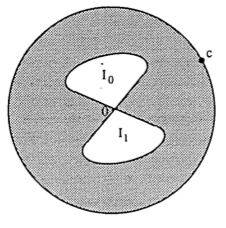
\includegraphics[scale=.4]{lobes1.png}
\end{figure}



Where each 'lobe' is mapped diffeomorphically (continuously bijected) to $C$.

\end{frame}


%%%%%%%%%%%%%%%%%%%%%%%%%%%%%%%%%%%%%%%%%%%%%%%%%%%%%%
%%%%%%%%%%%%%%%%%%%%%%%%%%%%%%%%%%%%%%%%%%%%%%%%%%%%%%
\subsection{frame 4}
\begin{frame}

Repeating this process yields nested lobes, each a diffeomorphism to its 'parent' lobe from the previous iteration. Below is a visualization of this process for two backwards-iterations.

\pause

\begin{figure}
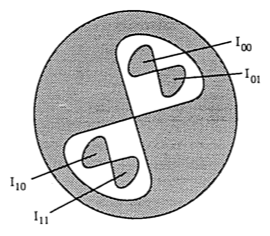
\includegraphics[scale=.4]{lobes2.png}
\end{figure}

\end{frame}


%%%%%%%%%%%%%%%%%%%%%%%%%%%%%%%%%%%%%%%%%%%%%%%%%%%%%%
%%%%%%%%%%%%%%%%%%%%%%%%%%%%%%%%%%%%%%%%%%%%%%%%%%%%%%
\subsection{frame 4}
\begin{frame}

Each lobe of the $k^{\text{th}}$ iteration of this process can be identified by a $0$ or $1$, as each lobe 
diffeomorphically maps to two inner lobes during each iteration. 

\vspace{.4cm}
\pause

We therefore have $2^k$ unique lobes after $k$ iterations.

\vspace{.4cm}
\pause

Define
\begin{align*}
I_{s_0s_1\ldots s_n} = \{z\in D \; | \;  z \in I_{s_0}, Q_c(z) \in I_{s_1}, \ldots, Q_c^{\circ n}(z) \in I_{s_n}\}
\end{align*}

\pause

As you may have noticed, this is identical to our previous use of symbolic dynamics (in relation
to the Cantor Middle-Thirds set). By similar logic to our discussion before, the following  
intersection is a nonempty set.
\begin{align*}
\bigcap\limits_{n\ge 0} I_{s_0s_1 \ldots s_n}
\end{align*}



\end{frame}


%%%%%%%%%%%%%%%%%%%%%%%%%%%%%%%%%%%%%%%%%%%%%%%%%%%%%%
%%%%%%%%%%%%%%%%%%%%%%%%%%%%%%%%%%%%%%%%%%%%%%%%%%%%%%
\subsection{frame 5}
\begin{frame}

This gives us that, for any $z \in \cap_{n\ge 0} I_{s_0s_1\ldots s_n}$, $Q_c^{\circ k} (z) \in D$ for all $k$. Hence, $z \in K_c$.

\vspace{0.4cm}
\pause

A \textsl{component} of $K_c$ is defined as an infinite intersection of figure-eights and their lobes. Two components are necessarily disjoint.

\vspace{0.4cm}
\pause

Conversely, any $z \in K_c$ must lie in exactly one of these components, since any infinite string of $1$s and $0$
maps to any $z$ by $S(z) = s_0s_1\ldots s_n$ provided $z\in \cap_{n\ge 0} I_{s_0s_1 \ldots s_n}$.

\vspace{0.4cm}
\pause

Similar arguments to those we used for the Cantor set yield that [1] this correspondence is continuous and [2] that each of these infinite intersections is exactly a single point in the complex plane. The mechanics behind this exceed the scope of this lecture (and class), so we will not include them here.



\end{frame}




%%%%%%%%%%%%%%%%%%%%%%%%%%%%%%%%%%%%%%%%%%%%%%%%%%%%%%
%%%%%%%%%%%%%%%%%%%%%%%%%%%%%%%%%%%%%%%%%%%%%%%%%%%%%%
\subsection{frame 6}
\begin{frame}


\begin{rmk}
$Q_c$ is supersensitive on $J_c$. (As handwavy as Devaney)
\end{rmk}


\begin{rmk}
Since $K_c$ is a Cantor set (each component of $K_c$ is a point) when $|c| > 2$, the Julia and filled Julia sets are identical ($K_c = J_c$).
\end{rmk}

\begin{rmk}
When $|c| > 2$, the orbit of 0 tents to $\infty$. This will be important on Thursday.
\end{rmk}

\end{frame}



%%%%%%%%%%%%%%%%%%%%%%%%%%%%%%%%%%%%%%%%%%%%%%%%%%%%%%
%%%%%%%%%%%%%%%%%%%%%%%%%%%%%%%%%%%%%%%%%%%%%%%%%%%%%%
\section{\scshape $K_c$ Algorithm}

\subsection{frame 2}
\begin{frame}

\begin{algorithm}[H]
  \SetKwFunction{KwPaint}{paintBlack} 
  \SetKwFunction{KwMax}{max} 
  \DontPrintSemicolon
  \LinesNumbered

\KwIn{grid, a list of evenly-spaced complex numbers in a rectangular region of the complex plane}

\For{$j  \leftarrow 1$ to $N$}{
	\For{$z$ in $grid$}{
		$z \leftarrow Q_c(z)$ \;
	}
}
		\tcp*{Shade all points which didn't escape}
\For{$z$ in $grid$} {
	\If{$|z| \le max(|c|,2)$}{
		\KwPaint{z}\;
	}
}
\caption{Algorithm to plot $K_c$ }
\end{algorithm}

\end{frame}


%%%%%%%%%%%%%%%%%%%%%%%%%%%%%%%%%%%%%%%%%%%%%%%%%%%%%%
%%%%%%%%%%%%%%%%%%%%%%%%%%%%%%%%%%%%%%%%%%%%%%%%%%%%%%


\subsection{frame 3}
\begin{frame}

\href{http://acko.net/blog/how-to-fold-a-julia-fractal/}{Acko -- How to Fold a Julia Fractal}

\end{frame}


%%%%%%%%%%%%%%%%%%%%%%%%%%%%%%%%%%%%%%%%%%%%%%%%%%%%%%
%%%%%%%%%%%%%%%%%%%%%%%%%%%%%%%%%%%%%%%%%%%%%%%%%%%%%%
\section{\scshape $J_c$ Algorithm}

\begin{frame}

Explanation for an alternative plotting algorithm

The above algorithm works well for $K_c$ but as well for $J_c$.
To remedy this, recall that $Q_c$ is supersensitive on $J_c$.
This means that any neighborhood $B$ of some point $z\in J_c$ has
the property that 
$\bigcup_{n=0}^\infty Q_0^{\circ n} (B) = \mathbb{C} \setminus \{p\}$ for at most one point $p$.

So supersensitive points serve as ``attractors'' for the backward iteration of $Q_c$, 
in the sense that for each supersensitive point, all of $\mathbb{C}$ except at most one point
must come arbitrarily close to it on reverse iteration. 


\end{frame}


%%%%%%%%%%%%%%%%%%%%%%%%%%%%%%%%%%%%%%%%%%%%%%%%%%%%%%
%%%%%%%%%%%%%%%%%%%%%%%%%%%%%%%%%%%%%%%%%%%%%%%%%%%%%%
\subsection{frame 2}
\begin{frame}

\begin{algorithm}[H]
  \SetKwFunction{KwRand}{randomBit} 
  \SetKwFunction{KwPaint}{paintBlack} 
  \SetKwFunction{KwRandC}{randomComplexNumber} 
  \DontPrintSemicolon
  \LinesNumbered
\KwIn{MaxIter, the maximum number of iterations to perform}


$z \leftarrow $ \KwRandC{}\;
\For{$j  \leftarrow 1$ to \ArgSty{MaxIter}}{
	$binaryRand \leftarrow $ \KwRand{} \;

		\tcp*{Pick a random backwards iteration}	
	\If{$binaryRand = 0$}{
		$z \leftarrow \sqrt{(z-c)}$\;
	} \Else{
		$z \leftarrow -\sqrt{(z-c)}$\;
	}

		\tcp*{Don't plot stray points}
	\If{$j > 100$}{
		\KwPaint{z}   \;
	}


}

\caption{Algorithm to plot $J_c$ }

\end{algorithm}

\end{frame}

%%%%%%%%%%%%%%%%%%%%%%%%%%%%%%%%%%%%%%%%%%%%%%%%%%%%%%
%%%%%%%%%%%%%%%%%%%%%%%%%%%%%%%%%%%%%%%%%%%%%%%%%%%%%%
\subsection{frame 3}
\begin{frame}

\end{frame}


%%%%%%%%%%%%%%%%%%%%%%%%%%%%%%%%%%%%%%%%%%%%%%%%%%%%%%
%%%%%%%%%%%%%%%%%%%%%%%%%%%%%%%%%%%%%%%%%%%%%%%%%%%%%%
\section{\scshape Pictures}

\begin{frame}


\href{http://demonstrations.wolfram.com/JuliaSetsAndTheMandelbrotSet/}{A demo of Julia-Mandelbrot correspondence}

\vspace{.4cm}

\href{http://www.juliasets.dk/UFP.htm}{Some pictures of generalized Julia sets}




\end{frame}


\end{document}












